\section{ХОД РАБОТЫ}
\subsection{Индивидуальное задание}

Требуется создать консоль администратора локальной сети класса С,
и консоли администраторов подсетей локальной сети \texttt{192.168.100.0}.

Консоль администратора локальной сети должна содержать оснастку «Управление компьютером»
и панель задач, обеспечивающую запуск всех четырех консолей администраторов подсетей.
Консоль каждого из администраторов подсетей должна содержать оснастку
<<Локальные пользователи и группы>> и панели задач,
обеспечивающие запуск программ MS Office Word и Total Commander.


\subsection{Разбиение локальной сети на четыре подсети}

Разобьем локальную сеть класса С \texttt{192.168.100.0} на четыре подсети.
Для получения четырёх сетей необходимо использовать два старших бита
последнего (четвёртого) байта. При этом маска подсети будет
иметь вид \texttt{255.255.255.192}.

В результате разбиения получаем следующие четыре подсети:
\begin{itemize}
 \item первая подсеть \texttt{192.168.100.0}
 \item вторая подсеть \texttt{192.168.100.64}
 \item третья подсеть \texttt{192.168.100.128}
 \item четвёртая подсеть \texttt{192.168.100.192}
\end{itemize}


\newpage
\subsection{Создание консолей подсетей}

Для создания новой консоли в меню <<Пуск>> необходимо выбрать пункт <<Выполнить>>,
ввести \texttt{mmc} и нажать <<OK>>. Появится окно, изображенное
на рисунке~\ref{pic:mmc_opened}.
\begin{figure}[h!]
  \centering
  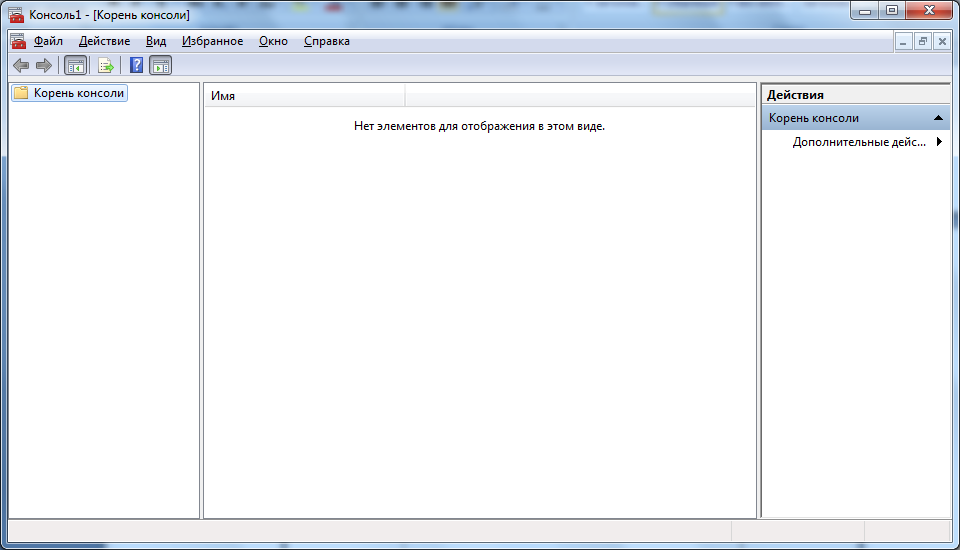
\includegraphics[width=0.8\linewidth]{pic/mmc_opened}
  \caption{Создание новой консоли в подсети}
  \label{pic:mmc_opened}
\end{figure}


В меню «Консоль (Console)» необходимо выбрать пункт
«Добавить/удалить оснастку (Add/Remove Snap-in)».
Откроется окно «Добавить/Удалить оснастку».
После нажатия кнопки «Добавить (Add)», на экране появится
окно «Добавить изолированную оснастку (Add Stand-alone Snap-in)» со списком
изолированных оснасток, имеющихся в системе. Выполнив двойной щелчок
на пункте «Локальные пользователи и группы», появится окно с
конфигурационными опциями для данной оснастки.
Необходимо оставить переключатель в положении
«локальным компьютером» (Local computer).
Затем нажать кнопку «Готово (Finish)» и кнопку «Закрыть» в окне
«Добавить изолированную оснастку». По окончании процедуры нажать кнопку «ОК».
Далее следует закрыть окно добавления оснасток, нажав кнопку «ОК».

Теперь окно консоли содержит оснастку «Локальные пользователи и группы».
Сохраним созданный инструмент с именем 192.168.100.0, выбрав пункт «Сохранить как (Save as)».
Для создания панели задач необходимо выполнить следующее:
\begin{enumerate}
\item В меню «Действие (Action)» или в контекстном меню любого узла
в окне консоли выбрать пункт «Новый вид панели задач (New Taskpad View)»,
откроется окно «Мастера создания вида панели задач (New Taskpad View Wizard)».
Нажать кнопку «Далее».
\item В следующем окне мастера выбрать стиль отображения и размер панели задач.
\item В следующем окне нужно ввести имя и описание создаваемой панели задач.
\end{enumerate}

Запустится «Мастер создания задач (New Task Wizard)»,
который «потребует» указать функцию задачи.

На панели задач требуется обеспечить запуск MS Word и Total Commander.
Поэтому необходимо выбрать пункт «Команда операционной системы».

В следующем окне требуется выбрать путь к запускаемой команде «MS Word».
Далее в появившемся окне нужно указать название задания и выбрать
значок для созданной задачи. В следующем окне для добавления задачи
запуска «Total Commander» нужно выбрать флажок «После нажатия кнопки «Готово»
снова запустить этот мастер».
Вновь запустится «Мастер создания задач (New Task Wizard)»,
который «потребует» указать функцию задачи.
Нужно снова выбрать пункт «Команда операционной системы».

В следующем окне выбрать путь к запускаемой команде «Total Commander».
Далее в появившемся окне нужно указать название задания и выбрать значок
для созданной задачи. Появится окно «Завершение мастера создания задач».
Нажав кнопку «Готово».


Аналогичным образом необходимо проделать аналогичные действия для создания
трёх оставшихся подсетей: \texttt{192.168.100.64}, \texttt{192.168.100.128},
\texttt{192.168.100.192}.

\subsection{Создание консоли администратора сети}

Консоль администратора локальной сети должна содержать оснастку «Управление компьютером»
и панель задач, обеспечивающую запуск всех четырех консолей администраторов подсетей.
Но перед этим этапом требуется создать четыре файла с расширением \texttt{.bat}
для того, чтобы можно было запускать созданные ранее консоли администраторов
локальных сетей. Создадим файл с расширением \texttt{.bat} «192.168.100.0.bat».
На рисунке~\ref{lst:192_168_100_0} приведено содержимое файла \texttt{192.168.100.0.bat}.

\begin{lstlisting}[caption={Содержимое файла \texttt{192.168.100.0.bat}},
label=lst:192_168_100_0]
 call 192.168.100.0.msc
 exit
\end{lstlisting}

С помощью команды «call» вызывается консоль администратора
подсети «192.168.100.0». С помощью команды «exit» происходит закрытие командной
строки после закрытия вызванной консоли.

Далее требуется создать консоль администратора локальной сети.
Для этого необходимо выполнить определенные действия. В меню «Консоль (Console)»
нужно выбрать пункт «Добавить/удалить оснастку (Add/Remove Snap-in)».
Откроется окно «Добавить/Удалить оснастку». Нажав кнопку «Добавить (Add)»,
на экране появится окно «Добавить изолированную
оснастку (Add Stand-alone Snap-in)» со списком изолированных оснасток, имеющихся в системе.
Выполнив двойной щелчок на пункте «Управление компьютером»,
появится окно с конфигурационными опциями для данной оснастки.
Необходимо оставить переключатель в положении локальным компьютером (Local computer).
Затем нажать кнопку «Готово (Finish)» и, далее кнопку «Закрыть» в
окне «Добавить изолированную оснастку».

По окончании процедуры нужно нажать кнопку «ОК». Закрыть окно добавления оснасток,
нажав кнопку «ОК». Теперь окно консоли содержит оснастку «Управление компьютером».

Для создания панели задач требуется выполнить следующее: в меню «Действие (Action)»
или в контекстном меню любого узла в окне консоли выбрать пункт
«Новый вид панели задач (New Taskpad View)», откроется окно «Мастера создания
вида панели задач (New Taskpad View Wizard)». Нажать кнопку «Далее».
В следующем окне мастера выбрать стиль отображения и размер панели задач.
Далее  требуется ввести имя «Корень консоли» и описание создаваемой панели задач.
Запустится «Мастер создания задач (New Task Wizard)»,
который «потребует» указать функцию задачи.

Панель задач должна обеспечивать запуск всех четырех консолей администраторов подсетей,
которые созданы были заранее. Поэтому необходимо выбрать пункт «Команда операционной системы».
В следующем окне нужно выбрать путь к файлу, который запускает
консоль администратора подсети «192.168.100.0».
Далее в появившемся окне указать название задания и выбрать значок для созданной задачи.
В следующем окне для добавления следующих задач нужно выбрать флажок «После нажатия кнопки «Готово».

Аналогичным образом создаются на панели инструментов задачи для запуска
консолей администраторов подсетей \texttt{192.168.100.64}, \texttt{192.168.100.128},
\texttt{192.168.100.192}.

Результат проделанных операций приведен на рисунке~\ref{pic:results}.
\begin{figure}[h!]
  \centering
  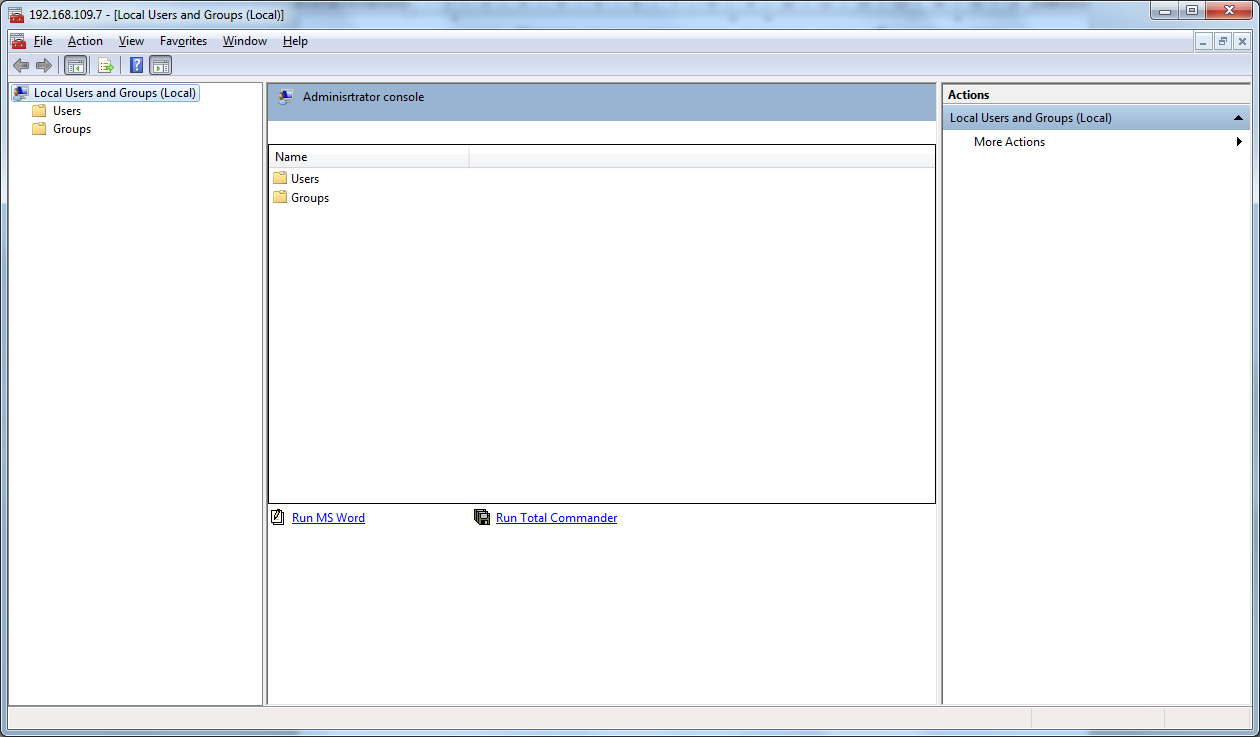
\includegraphics[width=0.8\linewidth]{pic/results}
  \caption{Окно <<Консоль администратора подсети>>}
  \label{pic:results}
\end{figure}
